\documentclass[11pt,a4,twosided,singlespacing,titlepagenumber=on]{scrreprt}

\usepackage[T1]{fontenc} % Handles accents etc better in the invisible details of the pdf output.
\usepackage[latin1]{inputenc} % May or may not be needed. Says that your *.tex file is a text file with ASCII latin1 encoding. You could use e.g. utf8 instead for easier accents etc.
\usepackage[UKenglish]{babel} % Let LaTeX know what language the text is in so it can select the correct hyphenation pattern etc

%%% American Mathematical Society packages
\usepackage{amsfonts,amssymb,amsmath,amsthm}
\usepackage{amsbsy}


\usepackage{algorithm}
\usepackage[noend]{algpseudocode}

%\usepackage{bm} % Possibly a better alternative to amsbsy for making bold typeface math.

%%% Graphics packages
\usepackage{graphicx}
%\graphicspath{{figures/}} % Useful if you have lots of images and want to keep thinks tidy by having a subfolder for images
%\usepackage{epstopdf} % If you produce your graphs as .eps files but then want to compile straight to PDF (e.g. because you are using TeXworks.) you may want to use this option. A better alternative of course would be to save all your graphs as *.pdf files from the start. Note that if you are compiling to pdf through PS/DVI then all your figures should be *.eps files and the epstopdf package should not be used.
%\usepackage{tikz} %For creating vector-graphics diagrams, flowcharts etc directly in LaTeX (takes some time to learn)
\usepackage[absolute]{textpos} % Used to position the Imperial College logo. You can comment this line and the next line out if you don't use the logo.
%\setlength{\TPHorizModule}{\paperwidth}\setlength{\TPVertModule}{\paperheight}
%\setlength{\TPHorizModule}{1cm}\setlength{\TPVertModule}{1cm}


%%% Referencing and cross-referencing
%\usepackage{color}
%\usepackage[colorlinks=false,linkcolor=red,urlcolor=cyan,citecolor=blue,breaklinks,plainpages=false,pdfpagelabels]{hyperref} % To make the hyperlinked cross-referencing visible.
\usepackage[colorlinks=false,pdfborder={0 0 0},plainpages=false,pdfpagelabels]{hyperref} % If you click on an item in the table of contents or a referenced equation/figure number, the PDF will go to the desired page. Neat isn't it?
\usepackage[round,authoryear,sort]{natbib} % Enable bibtex-based bibliography generation
%\usepackage[square,numbers,sort&compress]{natbib} % If you want numbered referencing instead of author-year style.



%%%%%%%%%%%%%%%%%%%%%%%%%%%%%%%%%%%%%
%%%%% Create or control Macros   %%%%%%%%%%%%%%%%%%%%
%%%%%%%%%%%%%%%%%%%%%%%%%%%%%%%%%%%%%

%\setcounter{secnumdepth}{3} %If you want subsubsections to be numbered
\numberwithin{equation}{chapter} % Reset equation numbers after each chapter.

%%% Theorem environments
\newtheorem{theorem}{Theorem}%[chapter]
\newtheorem{proposition}[theorem]{Proposition}%[chapter]
\newtheorem{definition}[theorem]{Definition}%[chapter]
\newtheorem{lemma}[theorem]{Lemma}%[chapter]
\newtheorem{corollary}[theorem]{Corollary}%[chapter]
%
\theoremstyle{remark}
\newtheorem{remark}[theorem]{Remark}%[chapter]
\newtheorem{example}[theorem]{Example}%[chapter]

%%% Potentially useful style changes:
%\renewcommand{\titlefont}{\normalcolor \normalfont \bfseries} %Change the title font from sans-serif to serif (the same font used for the rest of the document).
%\renewcommand*{\labelitemi}{$\bullet$} %Bullet points in the itemize environment.
%\renewcommand*{\tilde}{\widetilde} % Wider tildes
%\renewcommand*{\bar}{\overline} % Wider conjugate bars

%%% Examples of commands/macros that could be useful:
%\newcommand{\expectation}[1]{\mathbb{E}\left[ #1 \right]}
%\newcommand*{\setR}{{\mathbb R}}
%\newcommand{\commentify}[1]{} %Gives you an alternative way (other than %) to comment things out.
%%% These commands make it faster to get the correct roman font in equations: (similar to \exp, \cos, \sin etc). Alternatively yuo can always use e.g. $\mathrm{Var}$, but this is better.
%\DeclareMathOperator{\bigo}{O}
%\DeclareMathOperator{\littleo}{o}
%\DeclareMathOperator{\var}{Var}
%\DeclareMathOperator{\cov}{Cov}
%\DeclareMathOperator{\trace}{trace}
%\DeclareMathOperator{\sign}{sgn}
%\DeclareMathOperator{\rank}{rank}
%\DeclareMathOperator{\vecrm}{vec} % The \vec command already exists so you can't name this \vec.




%%%%%%%%%%%%%%%%%%%%%%%%%%%%%%%%%%%%%
%%%%% Define how to create the title page  %%%%%%%%%%%%%%%%
%%%%%%%%%%%%%%%%%%%%%%%%%%%%%%%%%%%%%
\makeatletter
\newcommand*{\supervisor}[1]{\gdef\@supervisor{#1}}
\newcommand*{\CID}[1]{\gdef\@CID{#1}}
\newcommand*{\logoimg}[1]{\gdef\@logoimg{#1}}
\renewcommand{\maketitle}{
\begin{titlepage}
\ifdefined\@logoimg
\begin{textblock*}{8cm}(1.75cm,1.75cm)
\includegraphics[width=70mm]{\@logoimg}
\end{textblock*}
\vspace*{1cm}
\else
%\vspace*{0cm}
\fi
\begin{center}
\vspace*{\stretch{0.1}}
Imperial College London\\
Derpartment of Mathematics\par
\vspace*{\stretch{1}} % This inserts vertical space and allows you to specify a relative size for the vertical spaces.
{\titlefont\Huge \@title\par} % If your title is long, you may wish to use \huge instead of \Huge.
\vspace*{\stretch{2}}
{\Large \@author \par}
\vspace*{1em}
{\large CID: \@CID \par}
\vspace*{\stretch{0.5}}
{\large Supervised by \@supervisor \par}
\vspace*{\stretch{3}}
{\Large \@date \par}
\vspace*{\stretch{1}}

\textit{This report is submitted as part requirement for the MSc Degree in Statistics at Imperial College London. It is substantially the result of my own work except where explicitly indicated in the text.
The report will be distributed to the internal and external examiners, but thereafter may not be
copied or distributed except with permission from the author.}
\vspace*{\stretch{0.1}}
\end{center}%
\end{titlepage}%
}
\makeatother


%%% And the abstract page
\renewenvironment{abstract}%
{\chapter*{Abstract}\thispagestyle{plain}}%
{\clearpage}
%%% And why not change the quote environment
\newenvironment{myquote}%
{\begin{quote}{\Large{}``}}%
{\ifhmode\unskip\fi{\Large{}''}\end{quote}}


\title{State Space Modelling for Statistical Arbitrage}
\author{Philippe~Remy}
\CID{00993306}
\supervisor{Nikolas Kantas and Yanis Kiskiras}
\date{\today}
\logoimg{Imperial__4_colour_process.jpg}

\begin{document}


\maketitle

\declaration

\begin{abstract}
This project is aimed to investigate the practical benefit of using more complex modelling than what is currently standard practice in applications related to statistical arbitrage. The underlying assets will be modelled using appropriate mean-reverting time series or state space models. In order to fit these models to real data the project will involve using advanced particle methods such as Particle Markov Chain Monte Carlo. The primary aim of the project is to assess whether using more advanced modelling and model calibration will result to better performance than simple models used often in practise. This will be illustrated in numerical examples, where the computed portfolio is used for a realistic scenario obtained by popular trading platforms. Simulations will be mainly run in Matlab, but embedding C/C++ routines may be required to speed up computations. The project is a challenging computational Statistics application to finance and is this suitable for a student with an interest in finance, very good apptitute to computing and understanding of the material in the course related to Monte Carlo methods and Time Series.
\end{abstract}
\newpage
%\chapter*{Acknowledgements}
%Thank you supervisor/friends/family/pet.
%\begin{myquote}
%Include an acknowledgement.
%\end{myquote}
%\newpage

% Automatically create a table of contents
\renewcommand{\contentsname}{Table of Contents}
\tableofcontents
\newpage

% Figure and table lists if you want them.
%\cleardoublepage
%\phantomsection
%\listoffigures 
%\addcontentsline{toc}{chapter}{\listfigurename}
%\newpage
%\phantomsection
%\listoftables  
%\addcontentsline{toc}{chapter}{\listtablename}
%\newpage


%\pagestyle{headings} % uncomment this if you want headers on your pages. Google fancyhdr or look into the options of scrreprt if you want different headers.
\chapter{State Space Modelling}
\section{Bootstrap Particle Filter}

The bootstrap particle filter is an iterative method for carrying out Bayesian inference for dynamic state space (partially observed Markov process) models, sometimes also known as hidden Markov models (HMMs). Here, an unobserved Markov process, $x_0,x_1,\ldots,x_T$ governed by a transition kernel $p(x_{t+1}|x_t)$ is partially observed via some measurement model $p(y_t|x_t)$ leading to data $y_1,\ldots,y_T$. The idea is to make inference for the hidden states $x_{0:T}$ given the data $y_{1:T}$. The method is a very simple application of the importance resampling technique. At each time, t, we assume that we have a (approximate) sample from $p(x_t|y_{1:t}$) and use importance resampling to generate an approximate sample from $p(x_{t+1}|y_{1:t+1}$).

More precisely, the procedure is initialised with a sample from $x_0^k \sim p(x_0),\ k=1,\ldots,M$ with uniform normalised weights ${w'}_0^k=1/M$. Then suppose that we have a weighted sample $\{x_t^k,{w'}_t^k|k=1,\ldots,M\}$ from $p(x_t|y_{1:t}$). First generate an equally weighted sample by resampling with replacement M times to obtain $\{\tilde{x}_t^k|k=1,\ldots,M\}$ (giving an approximate random sample from $p(x_t|y_{1:t}$)). Note that each sample is independently drawn from $\sum_{i=1}^M {w'}_t^i\delta(x-x_t^i)$. Next propagate each particle forward according to the Markov process model by sampling $x_{t+1}^k\sim p(x_{t+1}|\tilde{x}_t^k),\ k=1,\ldots,M$ (giving an approximate random sample from $p(x_{t+1}|y_{1:t}$)). Then for each of the new particles, compute a weight $w_{t+1}^k=p(y_{t+1}|x_{t+1}^k$), and then a normalised weight ${w'}_{t+1}^k=w_{t+1}^k/\sum_i w_{t+1}^i$.

It is clear from our understanding of importance resampling that these weights are appropriate for representing a sample from $p(x_{t+1}|y_{1:t+1})$, and so the particles and weights can be propagated forward to the next time point. It is also clear that the average weight at each time gives an estimate of the marginal likelihood of the current data point given the data so far. So we define

$$\displaystyle \hat{p}(y_t|y_{1:t-1})=\frac{1}{M}\sum_{k=1}^M w_t^k$$

and

$$\displaystyle \hat{p}(y_{1:T}) = \hat{p}(y_1)\prod_{t=2}^T \hat{p}(y_t|y_{1:t-1}).$$

Again, from our understanding of importance resampling, it should be reasonably clear that $\hat{p}(y_{1:T})$ is a consistent estimator of ${p}(y_{1:T}$). It is much less clear, but nevertheless true that this estimator is also unbiased. The standard reference for this fact is Del Moral (2004), but this is a rather technical monograph. A much more accessible proof (for a very general particle filter) is given in Pitt et al (2011).

It should therefore be clear that if one is interested in developing MCMC algorithms for state space models, one can use a pseudo-marginal MCMC scheme, substituting in \hat{p}_\theta(y_{1:T}) from a bootstrap particle filter in place of $p(y_{1:T}|\theta)$. This turns out to be a simple special case of the particle marginal Metropolis-Hastings (PMMH) algorithm described in Andreiu et al (2010). 

In bootstrap particle filter, $\pi(x_k^{(i)} | x_{0:k-1}^{(i)}, y_{0:k}) = p(x_k^{(i)}|x_{k-1}^{(i)})$. When the transition prior probability is used as the importance function, the weights update formula is simplified:

$$
w_k^{(i)} = w_{k-1}^{(i)} \frac{p(y_k|x_k^{(i)})p(x_k^{(i)}|x^{(i)}_{k-1})}{\pi(x_k^{(i)}|x^{(i)}_{0:k-1},y_{0:k})}= w_{k-1}^{(i)} p(y_k|x_k^{(i)})
$$ 

In the bootstrap particle filter, it is clear that the average weight at each time gives an estimate of the marginal likelihood of the current data point given the data so far:

$$ p^N_{\theta}(y_t | y_{0:t-1}) = \frac{1}{N} \sum_{k=1}^N w_t^k$$
The marginal likelihood at time $T$ is:
$$ p_{\theta}(y_{0:T}) = p(y_0)\prod_{t=1}^T p(y_t | y_{1:t-1})$$

Again, from our understanding of importance resampling, it should be reasonably clear that $\hat{p}^N_{\theta}(y_{0:T})$ is a consistent estimator of $p_{\theta}(y_{0:T})$. It is much less clear, but nevertheless true that this estimator is also unbiased according to Del Moral (2004).

The marginal log likelihood and its estimator are:
\begin{align*}
\log(p_{\theta}(y_{0:t})) &= \log(p(y_0)) + \sum_{t=1}^t \log \left(p(y_t | y_{1:t-1}) \right) \\
\log(p^N_{\theta}(y_{0:t})) &= - \log(N) + \sum_{t=1}^t \log \left(\frac{1}{N} \sum_{k=1}^N w_t^k \right)
\end{align*}

\begin{algorithm}
\caption{Bootstrap Particle Filtering Algorithm (SIR)}\label{euclid}
\begin{algorithmic}[1]
\Procedure{}{}
\\
\For{i from 1 to N} 
	\State $x_k^{(i)} \sim \pi(x_k | x_{0:k-1}^{(i)}, y_{0:k})$
	\State $w_k^{(i)} = \hat{w}_k^{(i-1)} p(y_k | x_k^{(i)})$
\EndFor{end}
\\
\For{i from 1 to N} 
	\State $w_k^{(i)} = \hat{w}_k^{(i)} / \sum_{j=1}^N \hat{w}_k^{(j)} $
\EndFor{end}
\\
\State $x_k$ = resampling($x_k$, $w_k)$
\For{i from 1 to N} 
	\State $w_k^{(i)} = 1 / N$
\EndFor{end}
\\
\EndProcedure
\Return $(x_k, w_k)$

\end{algorithmic}
\end{algorithm}

\newpage
\section{Stochastic Volatility}
\subsection{Simple SV Model}
The following scalar non-linear Hidden Markov model is considered:
\begin{align*}
  X_n &=  \rho X_{n-1} + \sigma V_n\\
  Y_n &=  \beta \exp \left( \frac{X_n}{2} \right) W_n
\end{align*}
where  $W_n, V_n \sim \mathcal{N}(0,1)$ iid and $X_0 \sim \mathcal{N} \left(0, \frac{\sigma^2}{1-\rho^2} \right)$. The model is non-linear because the component $Y_n$ has some non-additive noise and because it is non-linear with $X_n$. A bootstrap particle filter is derived with respect to this model. With little surprise, the SIR (Sequential Importance Sampling) Sequential Monte Carlo filter provides a better estimate than the SIS (Sequential Importance Sampling) filter. It is able to better track the peaks of the process $x^*_{0:T}$.

\section{PMMH}

In a more general context, a Metropolis Hastings scheme can be used to target $p(\theta| y)$ with the ratio:

\begin{align*}
\min \left( 1, \frac{p(\theta^\star)}{p(\theta)} \times  \frac{q(\theta|\theta^\star)}{q(\theta^\star|\theta)} \times \frac{p({y}|\theta^\star)}{p({y}|\theta)} \right)
\end{align*}

where $q(\theta^\star|\theta)$ is the proposal density. In Hidden Markov Models, the marginal likelihood $p(y|\theta)$ is often intractable and the ratio is hard to compute. The simple likelihood-free scheme targets the full joint posterior $p(\theta,x|y)$. Usually $p(x|\theta)$ is tractable. For instance, in the linear Gaussian case, $x_{0:T}$ can be simulated when $\rho$ and $\tau$ are known. The MH is built in two stages. First, a new $\theta^*$ is proposed from $q(\theta^\star|\theta)$ and then, $x^*$ is sampled from $p(x^\star|\theta^\star)$. The pair $(\theta^\star,x^\star)$ is accepted with the ratio:

\begin{align*}
\min \left( 1, \frac{p(\theta^\star)}{p(\theta)} \times  \frac{q(\theta|\theta^\star)}{q(\theta^\star|\theta)} \times \frac{p(y|{x}^\star,\theta^\star)}{p(y|{x},\theta)} \right)
\end{align*}
At each step, the $x^*$ is consistent of $\theta^*$ thanks to this proposed mecanism. The main drawback is that $T$ must be really small to have a good acceptance rate. As a matter of fact, since the conditional likelihood $p(y|{x}^\star,\theta^\star)$ is a product of $T$ terms over the path $x_{0:T}$, it becomes intractable very quickly as $T$ increases. The sampled $x^*$ must also be consistent with $y$. This is the reason why $x^*$ should be sampled from $p(x^\star|\theta^\star,y)$. The ratio becomes:

\begin{align*}
 \min \left(1, \frac{p(\theta^\star)}{p(\theta)}   \frac{p({x}^\star|\theta^\star)}{p({x}|\theta)}   \frac{f(\theta|\theta^\star)}{f(\theta^\star|\theta)}   \frac{p(y|{x}^\star,\theta^\star)}{p(y|{x},\theta)}  \frac{p({x}|y,\theta)}{p({x}^\star|y,\theta^\star)} \right)
\end{align*}

Using the basic marginal likelihood identity of Chib (1995), the ratio is simplified to:

\begin{align*}
 \min \left(1, \frac{p(\theta^\star)}{p(\theta)}  \frac{p(y|\theta^\star)}{p(y|\theta)} \frac{f(\theta|\theta^\star)}{f(\theta^\star|\theta)} \right)
\end{align*}
Remarkably $x$ is no more present and the ratio is exactly the same as the marginal scheme shown before. Indeed the ideal marginal scheme corresponds to PMMH when $N \rightarrow +\infty$. The likelihood-free scheme is obtained with just one particle in the filter. When $N$ is intermediate, the PMMH algorithm is a trade-off between the ideal and the likelihood-free schemes, but is always likelihood-free when one bootstrap particle filter is used.

\chapter{Then you get to the meaty stuff}
\begin{myquote}
The main sections should guide the reader through your results, analysing them and explaining them.
It should show both your successes and your failures in trying to solve your problem (your unsuccessful
attempts should be discussed, especially if you have ideas or explanations as to why they failed).
\end{myquote}
\section{With things like Methods}
It turns out that doing mathematics properly requires paying attention to many subtle details. For example
\begin{equation}
2=2+(1-1)=(2-1)+1=1+1.
\label{eq:obvious}
\end{equation}
Beware of the different mathematical fonts, and note that often punctuation should be included at the end of equations. For example, if you understand that 
\begin{equation*}
0=c\cdot o \cdot s^2 \cdot 0=\int_{-\pi}^\pi cos^2(x) dx \neq \int_{-\pi}^\pi \cos^2(x) \mathrm{d}x=\pi,
\end{equation*}
then your equations will look much nicer.
\begin{myquote}
Maths: In formulas use \verb|\exp| and not \verb|exp|.
\end{myquote}
\subsection{organised into subsections if you want}
Because well ordered thoughts are easier to follow.
\subsubsection{or even subsubsections}
And paragraphs. You most likely \emph{don't} want to use the \verb|\paragraph| command for this; just skip a line between paragraphs (or use \verb|\par| or \verb|\indent|).

You may wish to have a separate \verb|*.tex| file for each chapter, and use the \verb|\include{}| (or \verb|\input{}|) commands, if that helps you keep things organised. You can then use \verb|\includeonly{}| to only compile the chapter(s) you are currently working on.

\chapter{And yet more meaty stuff}
\begin{myquote}
You have to submit a thesis, a substantial written thesis normally not exceeding 12000 words. This is a
guideline: the appropriate length is a function of the project itself and its subject matter. Excess length
disproportionate to the content may be penalised.

The thesis should be on A4-sized paper and typed (ideally using LaTeX), and words or paragraphs
must not be crossed out. They should be in a simple binding; a ring or springback binder is suffcient. It
is important that students sign the declaration ``The work contained in this these is my own work unless
otherwise stated". Each thesis should include (i) a brief summary, (ii) an introduction (iii) the main body
of the thesis, and (iv) a bibliography.

Two printed copies of the thesis must be submitted to the MSc Administrator before the deadline listed
in Section 3. An electronic copy of the thesis (one PDF document) must also be submitted via the Virtual
Learning Environment. Late submission may be penalised and will normally delay consideration of the
thesis to the following year.
The thesis is worth 90\% of the project mark.
\end{myquote}

\begin{figure}[tbp] % Sometimes, you want your figure to appear in between the text you put before it and the text you put after it. h stands for `here' and does that.
\centering
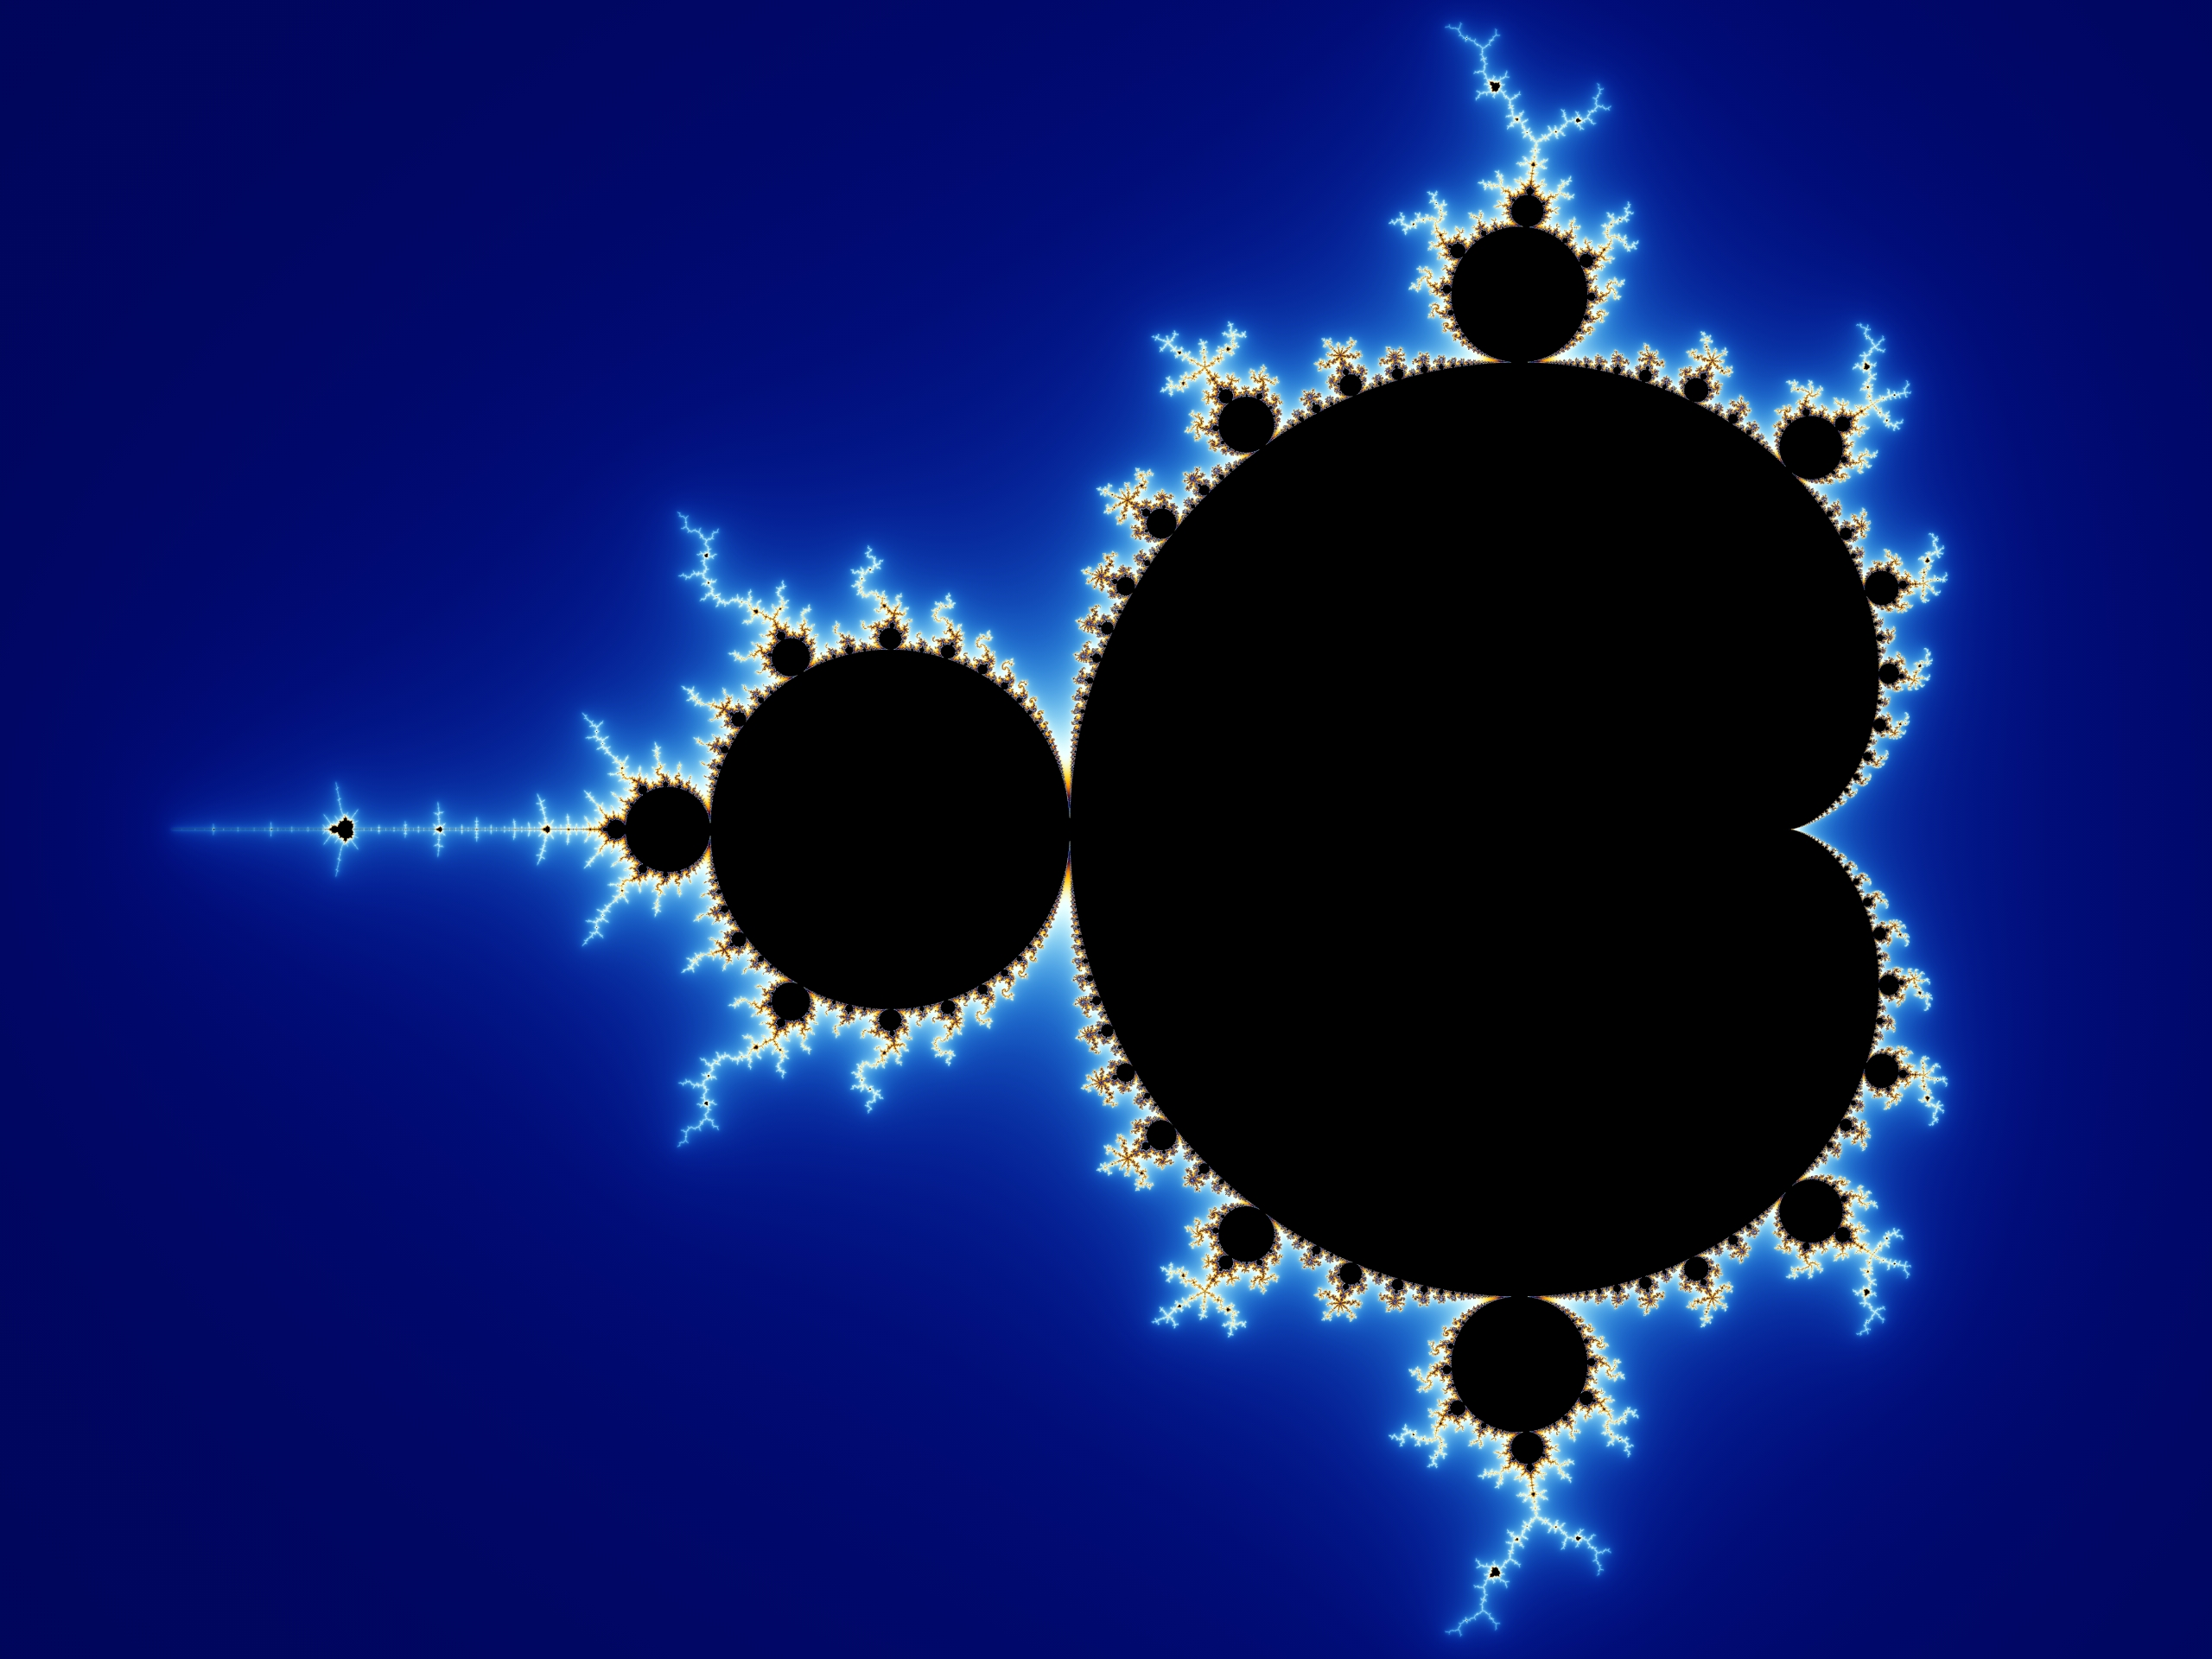
\includegraphics[width=0.8\textwidth]{mandelbrot.jpg} % You probably shouldn't use JPEG for graphs. Use the vector graphics formats EPS or PDF instead. If you really want a non-vector format then use PNG.

\caption{``Graphs
and simple diagrams (especially when they are neat) can sometimes be far more effective in presenting results
than lots of numbers and/or lots of words.''
{\small This figure is by Irina Pechkareva.}
\label{fig:mandelbrot}}
\end{figure}
%
\begin{myquote}
Figures: The best place is at the top or at the bottom of a page. If this is not possible they should go
on a separate page. In LaTeX this can be achieved by
\begin{verbatim}
\begin{figure}[tbp]
...
\end{figure}
\end{verbatim}
When generating plots from R it is usually best to export them as pdf or eps for inclusion in LaTeX. To get
Greek letters, sub and superscripts into labels use eg \verb|xlab=expression(alpha[5])|.
\end{myquote}

\chapter{Conclusion}
It's up to you whether you want your introduction/conclusion to be numbered chapters or not. (un-numbered chapters can be created with \verb|\chapter*{}|, but may require you to manually edit the table of contents (see the list of tables in the code comments or the bibliography for an example).

\begin{myquote}
The conclusion section should summarise what you have learned. If you would have done more, given
more time, you should indicate where your effort would have gone. If your work has raised any unsettled
questions, you should address them and indicate what further work needs doing.
\end{myquote}
\section{About Referencing}
The numbers in this sentence are clickable and refer to equation~(\ref{eq:obvious}) on page~\pageref{eq:obvious} and Figure~\ref{fig:mandelbrot}.

\begin{myquote}
List of references: Using author (year) style notation is good practice (the reader may know the paper, but
she will definitively not know the number in your reference list. To achieve this in LaTeX you can use BibTeX
together with the package natbib. If citing several references together, use \verb|\citep{ref1,ref2,ref3}|. Use
a coherent style - either all authors get their first full names or none gets their full names. Books need the
name of the publisher, journal articles need the name of the journal. When using BibTeX for generating
references, make sure that appropriate capitalisation is used, eg it should be Monte Carlo and not monte
carlo. To achieve this in BibTeX, use \verb|{M}onte {C}arlo|.
\end{myquote}

The bibliography below was generated by BibTeX using the natbib package. You should reference any material you use, e.g. journal articles \citep{cox_regression_1972}. For example \citet{mccullagh_generalized_1989} explain the theory of generalized linear models in their book. Not citing your sources usually constitutes plagiarism \citep{plagiarism}. I recommend using \verb|Ctrl+F| to search for question marks in your thesis, as these will often result from errors in referencing and cross-referencing \citep{nonexistingreference}.

There are various software options for managing references, which will allows you to automatically generate BibTeX files. Note however that some manual adjustments are typically required.

\cleardoublepage
\phantomsection
\addcontentsline{toc}{chapter}{\bibname} % Add an entry for the Bibliography in the Table of Contents
%\pagestyle{headings}
\bibliographystyle{abbrvnat} % set the bibliography style
\bibliography{bibtexfile} % generate the bibliography
%\bibliographystyle{abbrvnat} % <- Mistake in earlier version. After the bibliography is created it's too late to change the style.
% Pick a sensible bibliography style. 
% If like above you choose to use author-year style citations, you must choose a natbib-compatible bibliographystyle such as 'plainnat'. Abbrvnat is one of the few built-in styles of this type. You may find many more bibliography styles (*.bst files) online. You can also choose to write your bibliography manually instead of using BibTeX (This will take you longer, unless you plan to use the content of a BibTeX-generated *.bbl file as your starting point).
% When creating a BibTeX file using e.g. reference manager software, note that the entries may contain additional unwanted fields which you would then need to erase. For example, you probably don't want to include the URL of a journal paper in your bibliography.


%\cleardoublepage \fancyhead[L]{APPENDIX}
\appendix % This line declares that you are starting the appendix.
% If you want a single Appendix and want it to be called Appendix instead of Appendix A, the following should work:
%\setcounter{secnumdepth}{-1} %This turns off automatic chapter numbering
%\chapter{Appendix}

\chapter{You probably want to put things like computer programs and long boring proofs in an appendix}
\begin{myquote}
Any programs in the appendices should be representative. A copy of every single version of every code
is unnecessary. Programs should be documented with many comment lines and a discussion of the input
necessary to drive them and the output resulting from them as appropriate. Large tables of results should
be organised in reference form (as should large sets of graphs) with indices and tables of contents to guide
the interested reader through them. Appendices do not count towards the word limit.
\end{myquote}

There are better ways to include code than the example below, e.g. through the listings package (especially if you intend to print in colour). 
Although you could write your thesis in Sweave, I would not recommend it since it will make compilation slower.
\section{R code}
\begin{verbatim}
addone <- function(x) {
# This function inputs a numeric variable x
# and outputs x+1.
# If x is a non-negative integer, then it outputs the next positive integer.
  return(x+1)
}
\end{verbatim}
\chapter{More Guidelines}
\section{Titlepage}
\begin{myquote}
The title page is your own design however it should include your name, CID, project title, supervisor's
name. You may want to include the wording: ``Submitted in partial fulfilment of the requirements for the
MSc in Statistics of Imperial College London''. You should not be using the Imperial crest, but you can use
the Imperial logo:

\url{http://www3.imperial.ac.uk/graphicidentity/applyingthegraphicidentity/usingthecrest}

\url{http://www3.imperial.ac.uk/graphicidentity/applyingthegraphicidentity/usingthelogo}
\end{myquote}
The logo has been included in the current title design but must be downloaded into the same folder as your \verb|*.tex| file.

\section{Declaration}
\begin{myquote}
The second page must contain a signed and dated plagiarism statement, ``The work contained
in this thesis is my own work unless otherwise stated''. It is sufficient if you sign the hard copies.
\end{myquote}



\end{document}